\documentclass[12pt,letterpaper]{article}
\usepackage[utf8]{inputenc}
\usepackage{amsmath}
\usepackage{amsfonts}
\usepackage{amssymb}
\usepackage{graphicx}
\usepackage{hyperref}
\usepackage[space]{grffile}
\graphicspath{{/Users/jacob/Documents/My Stuff/Arduino/Shirt Folder/Shirt Folder/Design/Images/}}

\title{Shirt Folder}
\author{}
\date{}

\begin{document}
\maketitle
\section{Introduction}
This document describes the shirt-folding machine which I built. The shirt-folding machine is capable of folding most garments including shirts, shorts and pants. All files for the shirt folder can be found at \url{https://github.com/orangeturtle739/garmenttransporter/tree/master/Shirt\%20Folder}.

\section{Design}
The shirt folder consists of three flaps. Each flap is connected to a servo which can rotate the flap. Figure \ref{topview} shows a rendering of the shirt folder. Each of the flaps fold inward as shown in figure \ref{opentopview}.

The servos are connected to the flaps with a linkage consisting of wooden arms. Figure \ref{servolinkage} shows the linkage. When the button is hit, the shirt folder folds a shirt.

A SketchUp model of the shirt folder can be found at \url{https://github.com/orangeturtle739/garmenttransporter/blob/master/Shirt\%20Folder/Design/Shirt\%20Folder.skp}.

\section{Electronics}
Figure \ref{schematic} shows a schematic of the shirt folder's circuit. Every servo has its own 6V power supply and the Arduino Uno has a 9V power supply. All of the power supplies have their own switches and all of the grounds are connected together.

\section{Parts}
I used TowerPro 9805BB servos because they are able to provide lots of torque. For the main switch (labeled "Button" in figure \ref{topview}), I used a round push-on/push-off switch. For the Arduino switch and the servo switches, I used rocker switches.

\section{Use}
To use to shirt folder, install the program which can be found at \url{https://github.com/orangeturtle739/garmenttransporter/blob/master/Shirt\%20Folder/Shirt_Folder/Shirt_Folder.ino}. After installing the program, turn the Arduino on. Press the main switch twice (turn it on then off again) to initialize the servos. Then, place the shirt onto the shirt folder and press the main switch. Once the bottom flap has be activated, the folder will wait. Pull the shirt onto the bottom flap and press the main switch again. This will cause the bottom flap to rotate one more time which will complete the shirt folding.

\begin{figure}[ht]
  \centering
    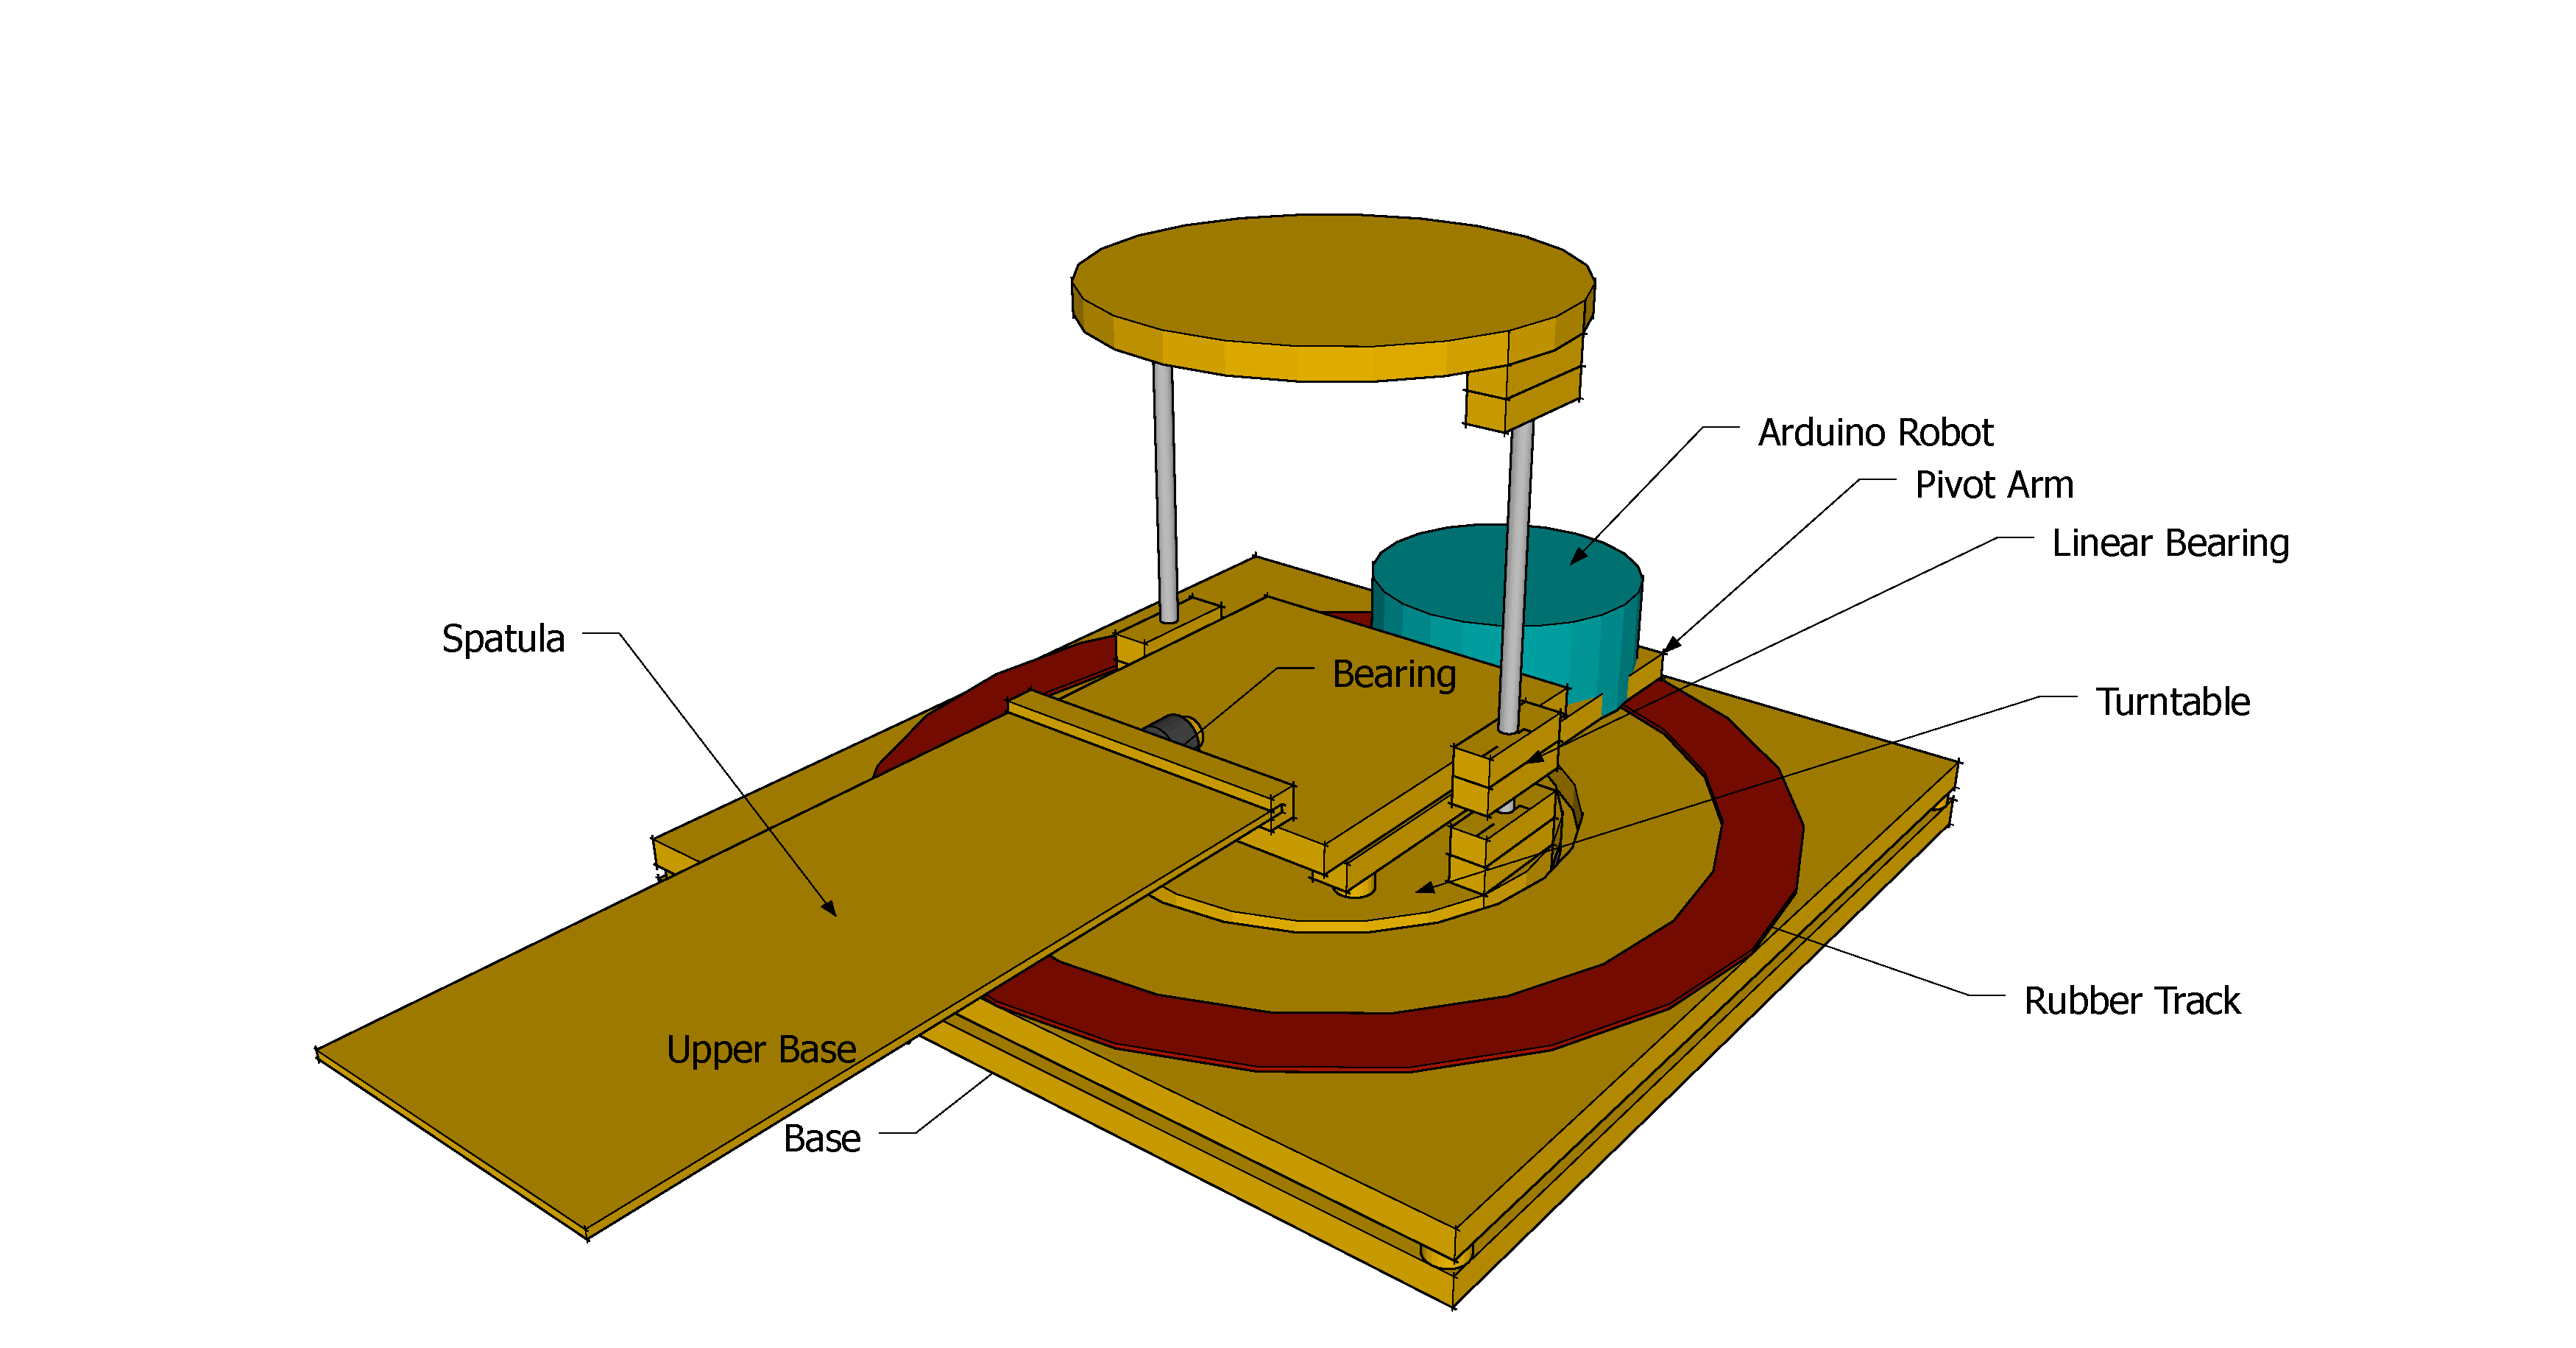
\includegraphics[width=\columnwidth]{Top View.pdf}
    \caption{Top view of shirt folder.}
    \label{topview}
\end{figure}
\begin{figure}[ht]
  \centering
    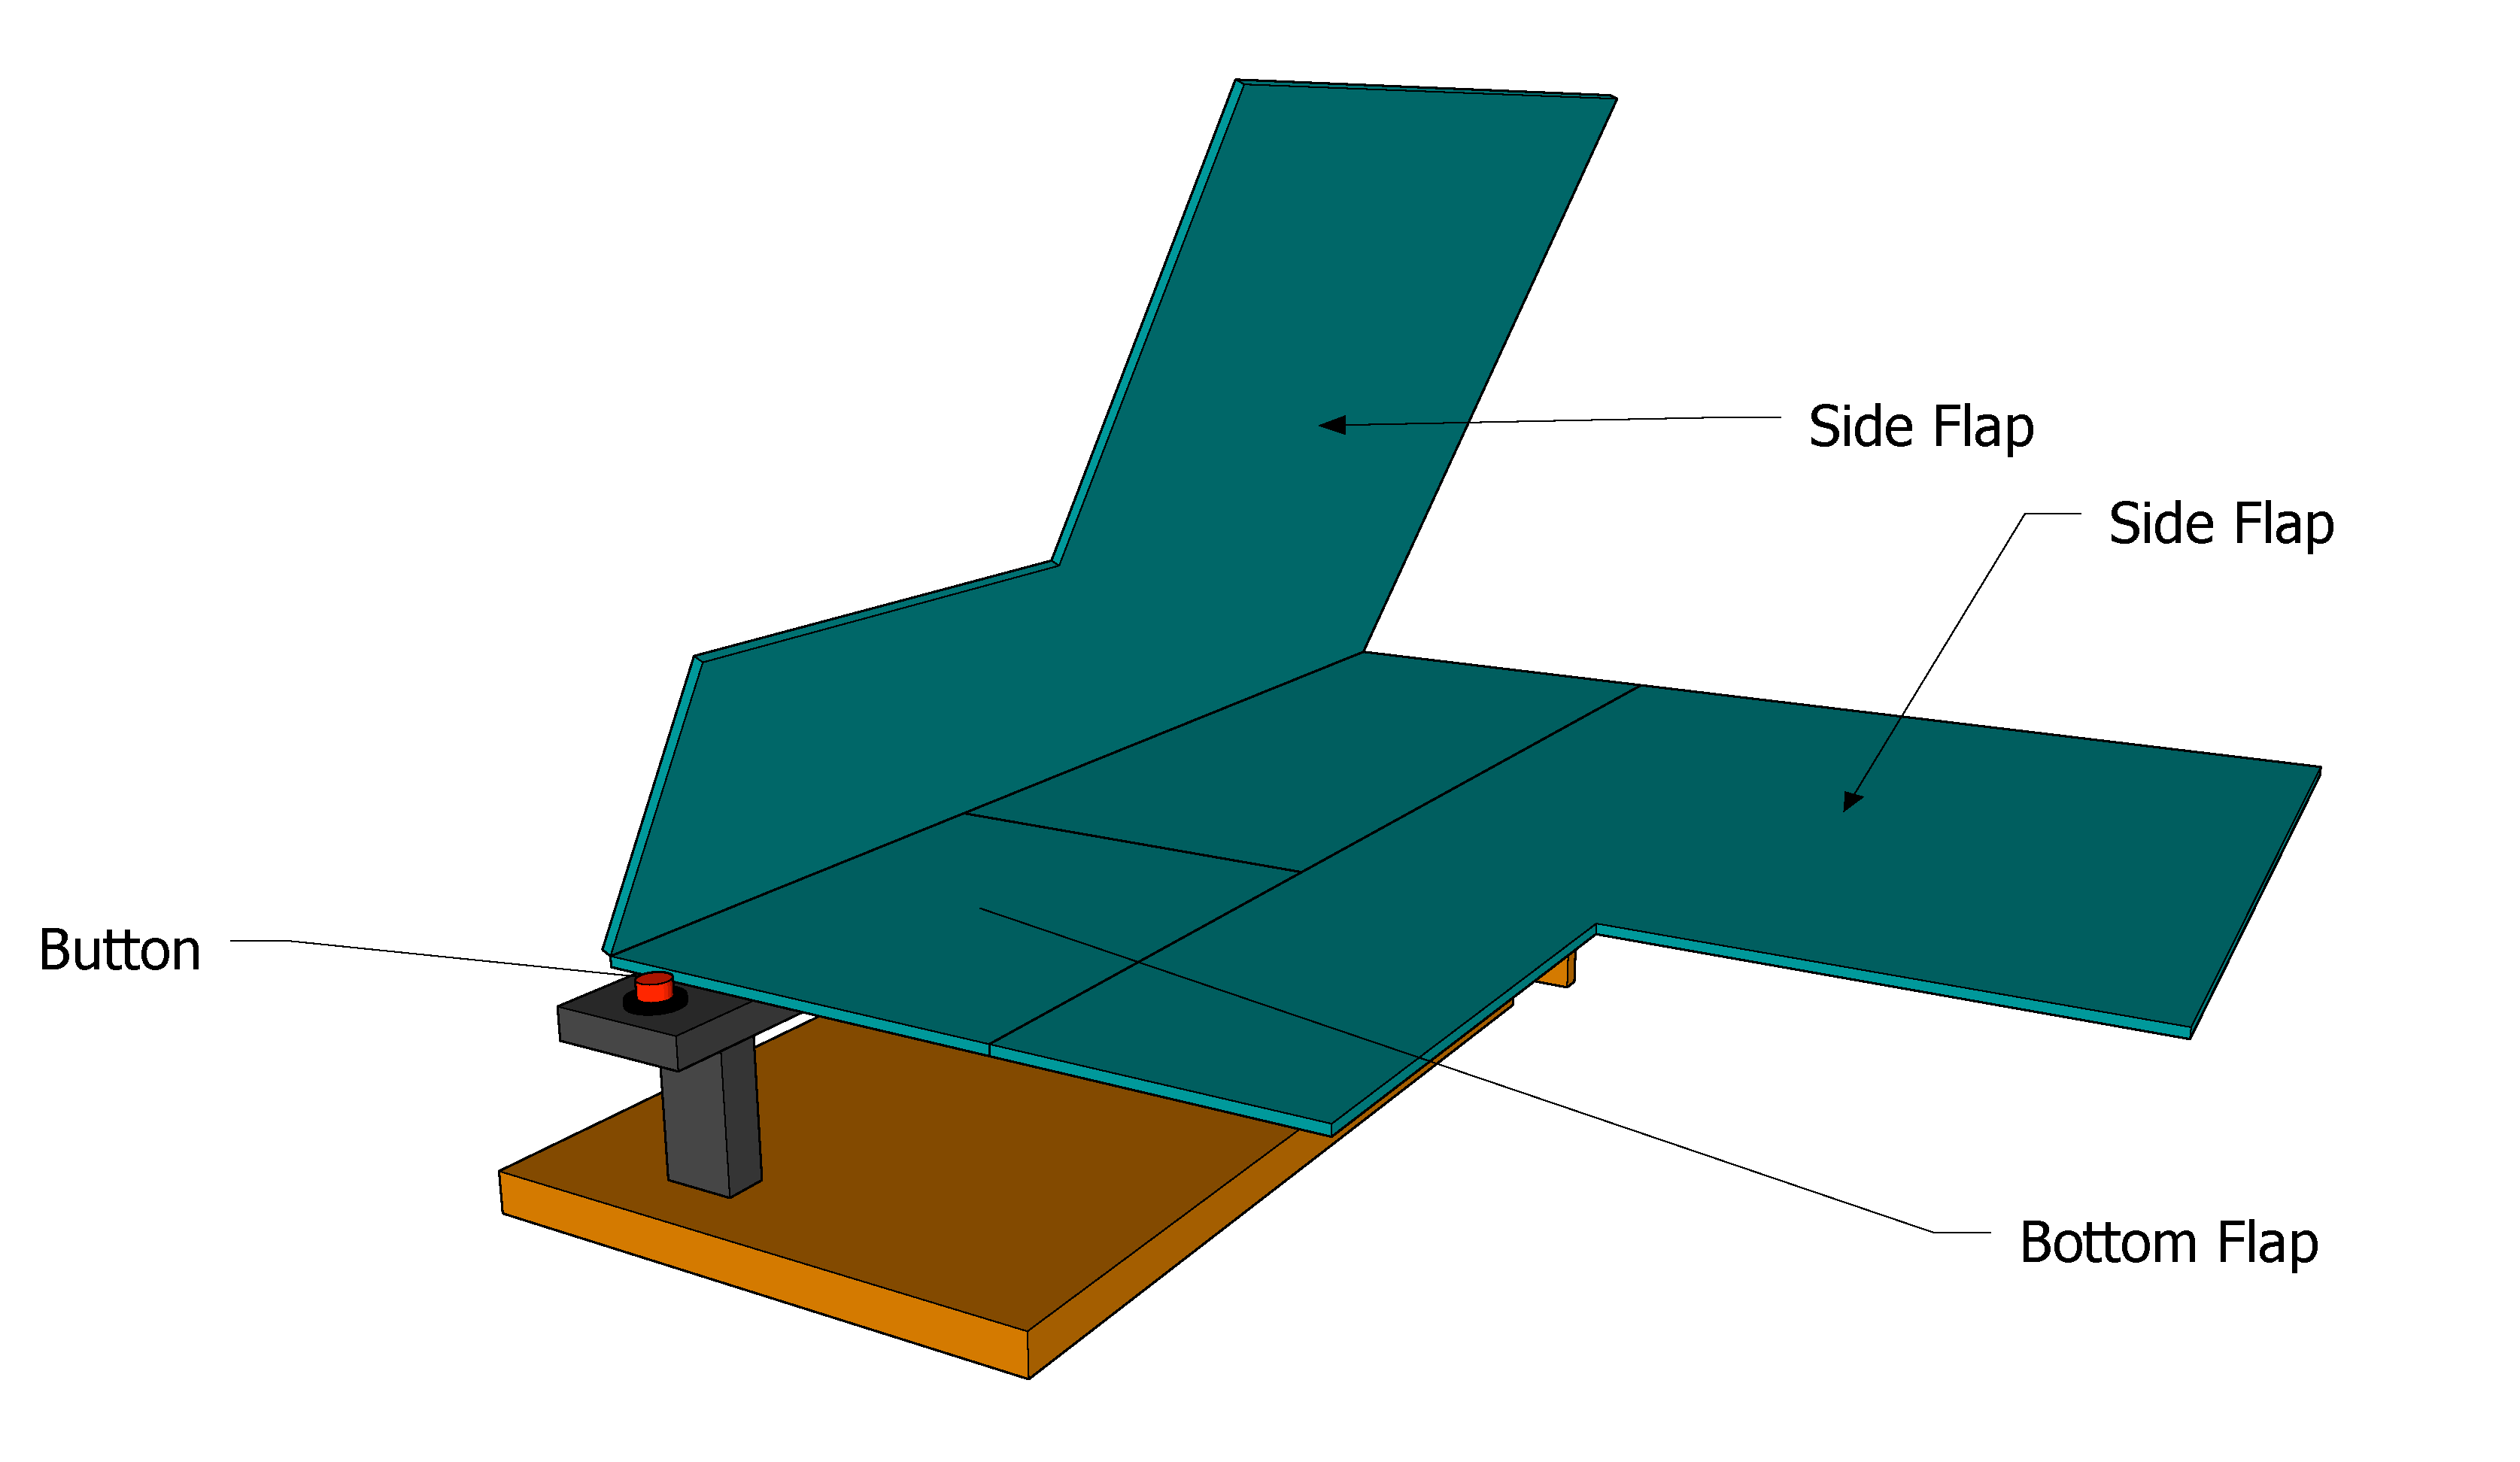
\includegraphics[width=\columnwidth]{Open Top View.pdf}
    \caption{Top view of shirt folder with one of the side flaps rotated.}
    \label{opentopview}
\end{figure}
\begin{figure}[ht]
  \centering
    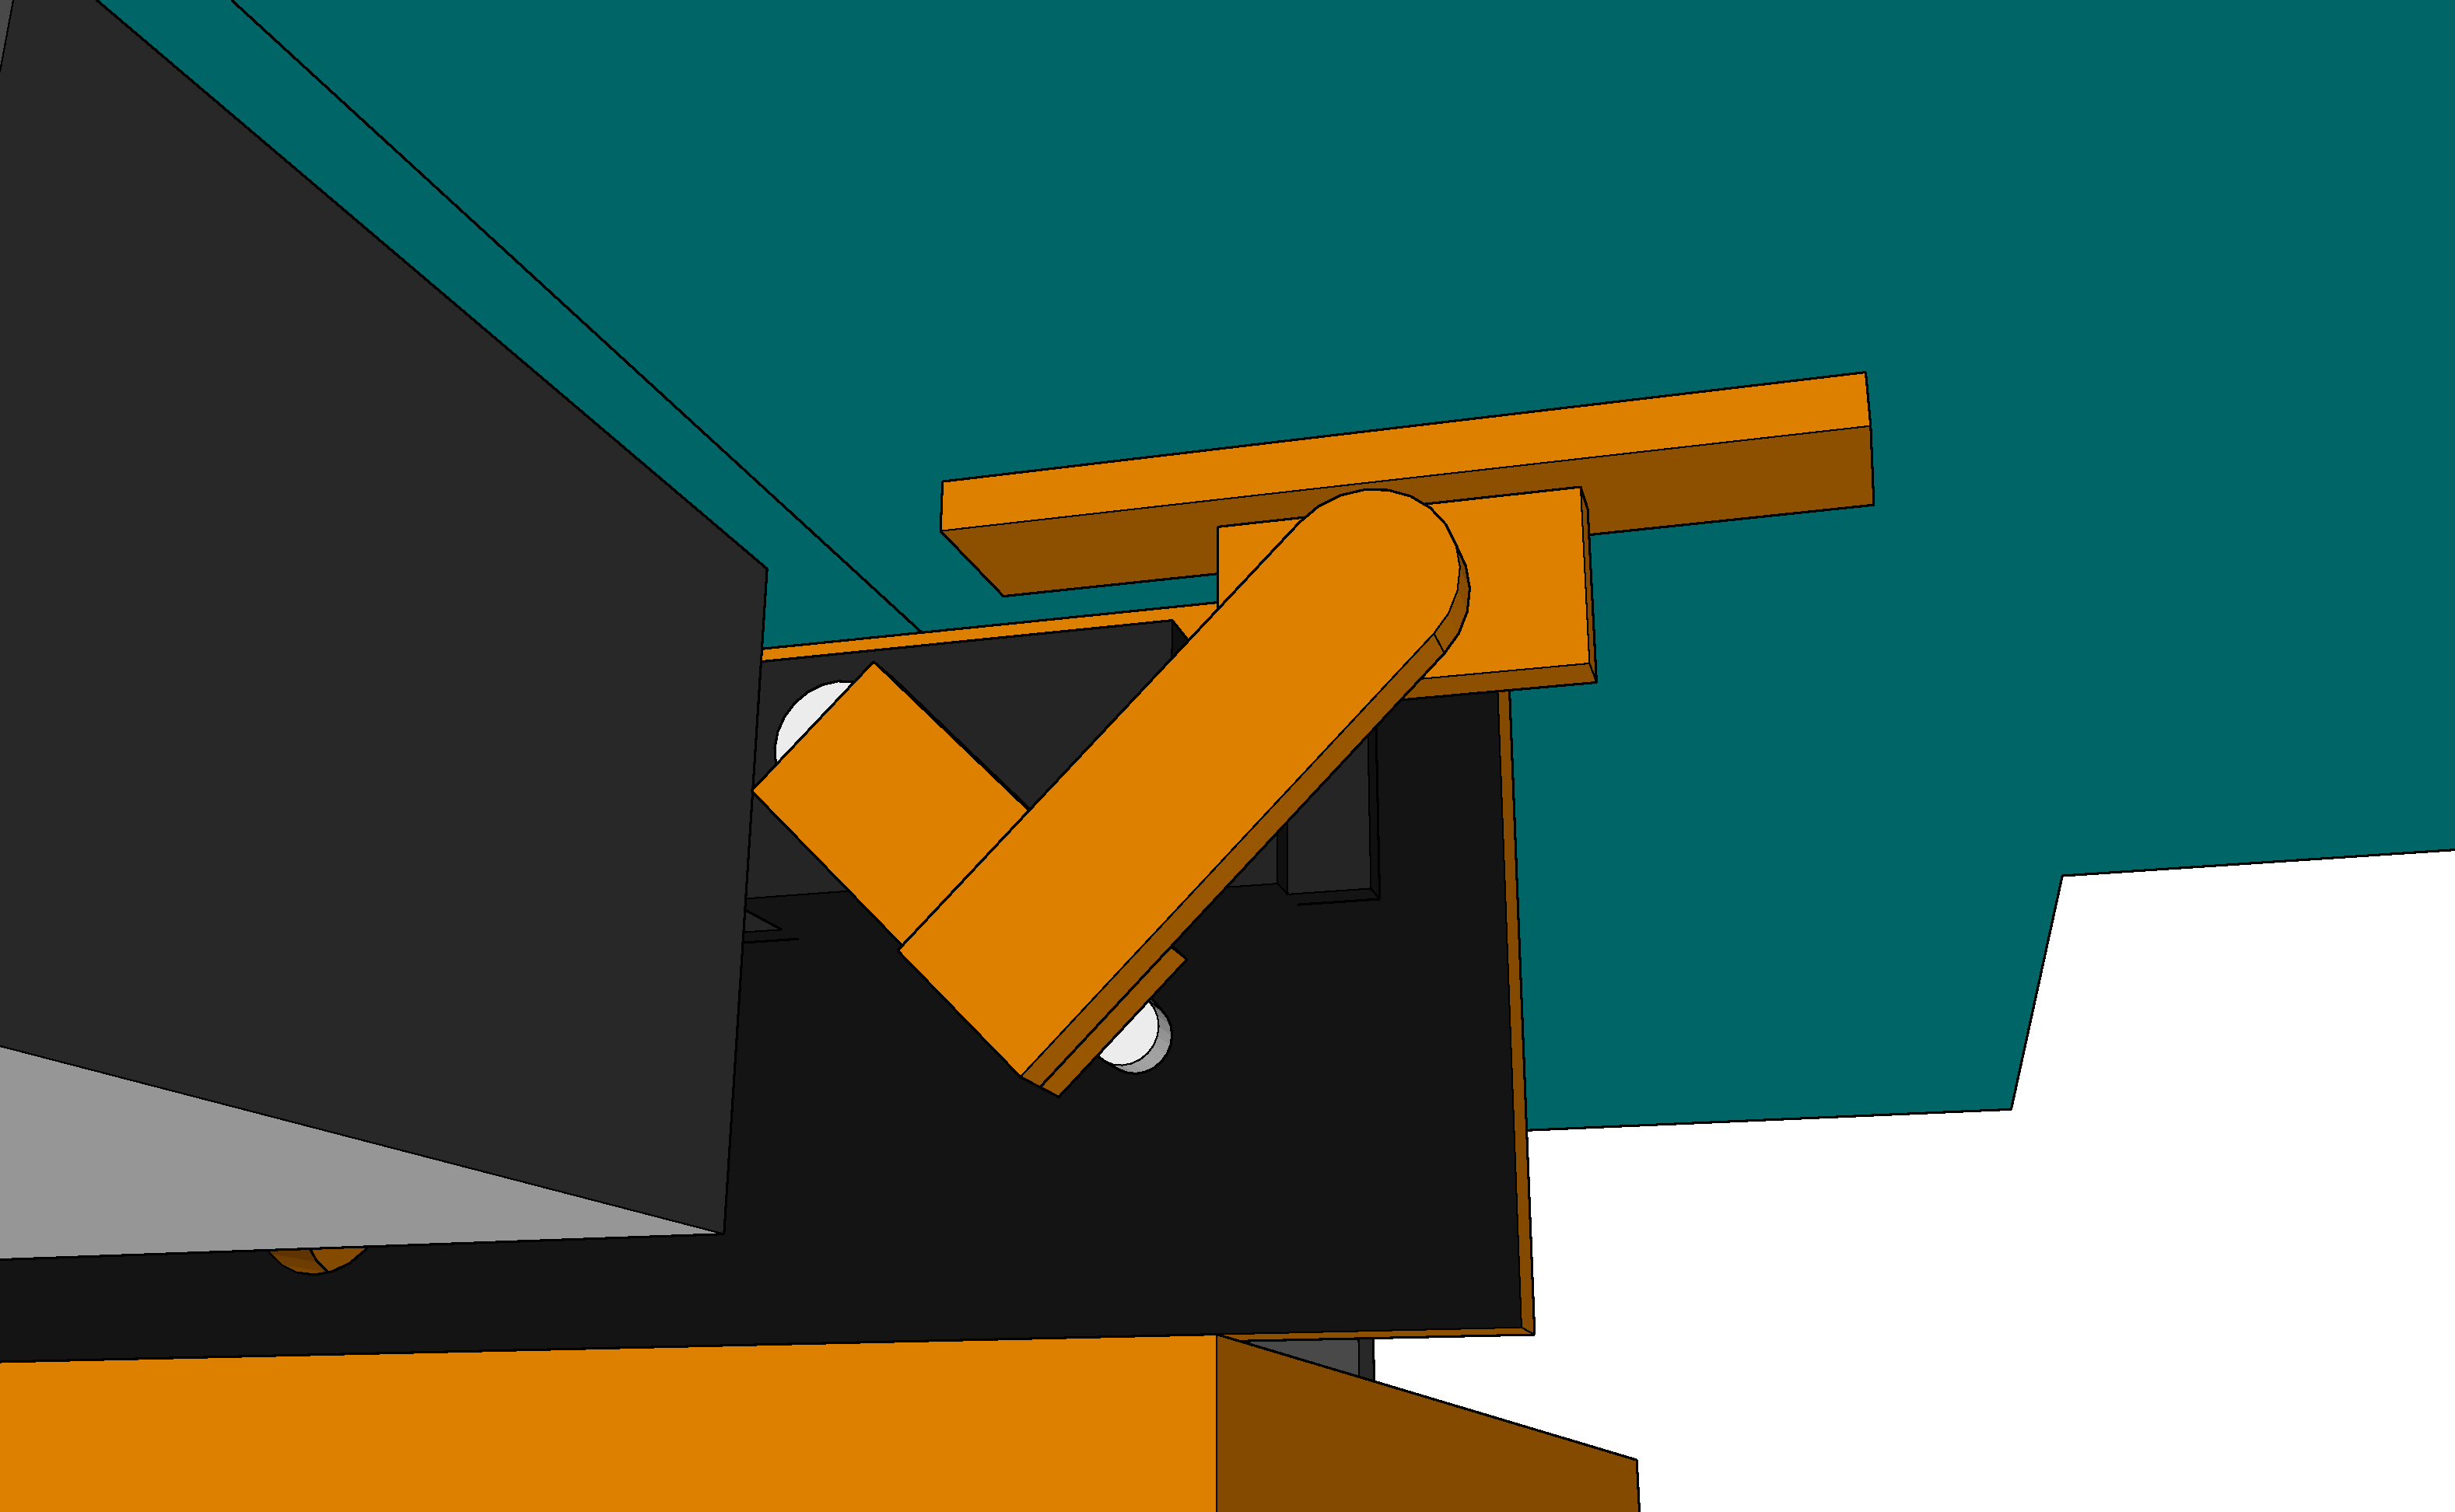
\includegraphics[width=\columnwidth]{Servo Linkage.pdf}
    \caption{The servo linkage.}
    \label{servolinkage}
\end{figure}
\begin{figure}[ht]
  \centering
    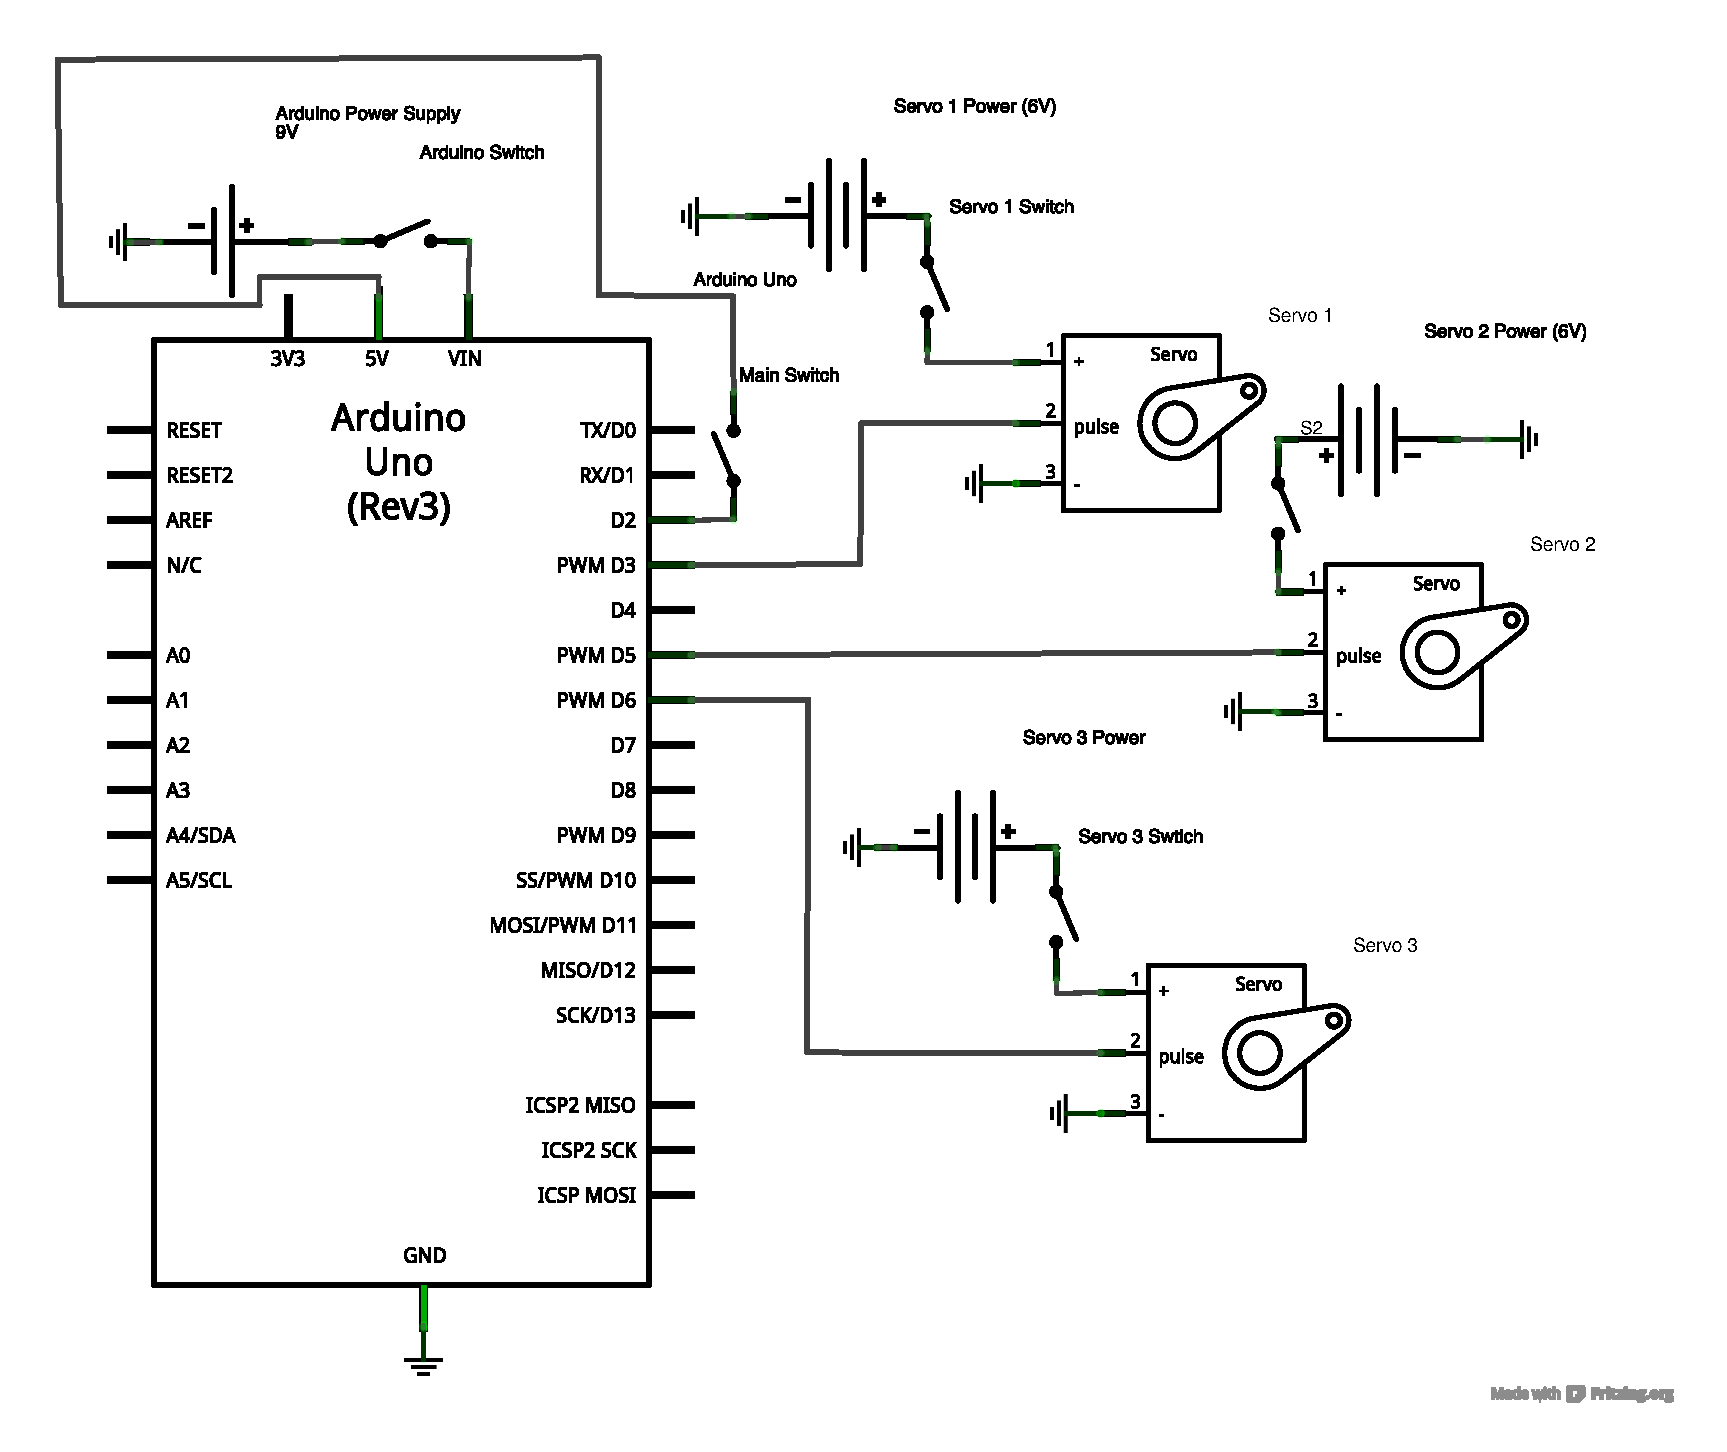
\includegraphics[width=\columnwidth]{Full Schematic.pdf}
    \caption{The schematic.}
    \label{schematic}
\end{figure}
\end{document}